
\section{Exploring institutionally curated cancer genomics data}\label{exploring-institutionally-curated-cancer-genomics-data}}


\subsection{The Cancer Genome Atlas}\label{the-cancer-genome-atlas}}

An overview of Bioconductor's resource for the Cancer
Genome Atlas (TCGA) is easy to obtain, with the
curatedTCGAData package.

\begin{Shaded}
\begin{verbatim}
library(curatedTCGAData)
tcgatab = curatedTCGAData(version="2.1.1")
\end{verbatim}
\end{Shaded}
%\begin{Shaded}
%\begin{Highlighting}[]
%\KeywordTok{library}\NormalTok{(curatedTCGAData)}
%\NormalTok{tcgatab =}\StringTok{ }\KeywordTok{curatedTCGAData}\NormalTok{(}\DataTypeTok{version=}\StringTok{"2.1.1"}\NormalTok{)}
%\end{Highlighting}
%\end{Shaded}

Records obtained for adrenocortical carcinoma (code ACC) are in Table \ref{tab:tab-lktab}.

\begin{table}

\caption{\label{tab:tab-lktab}Records returned by curatedTCGAData::curatedTCGAData(), filtered to those pertaining to adrenocortical carcinoma.}
\centering
\begin{tabular}[t]{lllll}
\toprule
  & ah\_id & title & file\_size & rdataclass\\
\midrule
1 & EH4737 & ACC\_CNASNP-20160128 & 0.8 Mb & RaggedExperiment\\
2 & EH4738 & ACC\_CNVSNP-20160128 & 0.2 Mb & RaggedExperiment\\
3 & EH4740 & ACC\_GISTIC\_AllByGene-20160128 & 0.2 Mb & SummarizedExperiment\\
4 & EH4741 & ACC\_GISTIC\_Peaks-20160128 & 0 Mb & RangedSummarizedExperiment\\
5 & EH4742 & ACC\_GISTIC\_ThresholdedByGene-20160128 & 0.2 Mb & SummarizedExperiment\\
\addlinespace
6 & EH4744 & ACC\_Methylation-20160128\_assays & 239.2 Mb & SummarizedExperiment\\
7 & EH4745 & ACC\_Methylation-20160128\_se & 6 Mb & RaggedExperiment\\
8 & EH4747 & ACC\_Mutation-20160128 & 0.7 Mb & SummarizedExperiment\\
9 & EH4748 & ACC\_RNASeq2Gene-20160128 & 2.7 Mb & SummarizedExperiment\\
10 & EH4750 & ACC\_RPPAArray-20160128 & 0.1 Mb & SummarizedExperiment\\
\addlinespace
414 & EH8118 & ACC\_miRNASeqGene-20160128 & 0.2 Mb & SummarizedExperiment\\
415 & EH8119 & ACC\_RNASeq2GeneNorm-20160128 & 5.4 Mb & SummarizedExperiment\\
\bottomrule
\end{tabular}
\end{table}

Various conventions are in play in this table. The ``title'' field is
of primary concern. The title string can be decomposed into
substrings with interpretation
\texttt{{[}tumorcode{]}\_{[}assay{]}-{[}date{]}\_{[}optional codes{]}}. The column \texttt{ah\_id} will be
explained in section \ref{hubs}, and entries in column
\texttt{rdataclass} will be discussed in section \ref{class} below.


\subsubsection{Tumor code resolution}\label{tumor-code-resolution}}

There are 33 different tumor types available in TCGA. The
decoding of tumor codes for the first ten in alphabetical order is
provided in Table \ref{tab:tab-deco}.

\begin{table}

\caption{\label{tab:tab-deco}Decoding TCGA tumor code abbreviations.}
\centering
\begin{tabular}[t]{ll}
\toprule
Code & Tumor.Type\\
\midrule
ACC & Adrenocortical Carcinoma\\
BLCA & Bladder Urothelial Carcinoma\\
BRCA & Breast Invasive Carcinoma\\
CESC & Cervical Squamous Cell Carcinoma and Endocervical Adenocarcinoma\\
CHOL & Cholangiocarcinoma\\
\addlinespace
CNTL & Controls\\
COAD & Colon Adenocarcinoma\\
DLBC & Lymphoid Neoplasm Diffuse Large B-cell Lymphoma\\
ESCA & Esophageal Carcinoma\\
FPPP & FFPE Pilot Phase II\\
\addlinespace
GBM & Glioblastoma Multiforme\\
HNSC & Head and Neck Squamous Cell Carcinoma\\
KICH & Kidney Chromophobe\\
KIRC & Kidney Renal Clear Cell Carcinoma\\
KIRP & Kidney Renal Papillary Cell Carcinoma\\
\addlinespace
LAML & Acute Myeloid Leukemia\\
LCML & Chronic Myelogenous Leukemia\\
LGG & Brain Lower Grade Glioma\\
LIHC & Liver Hepatocellular Carcinoma\\
LUAD & Lung Adenocarcinoma\\
\addlinespace
LUSC & Lung Squamous Cell Carcinoma\\
MESO & Mesothelioma\\
MISC & Miscellaneous\\
OV & Ovarian Serous Cystadenocarcinoma\\
PAAD & Pancreatic Adenocarcinoma\\
\addlinespace
PCPG & Pheochromocytoma and Paraganglioma\\
PRAD & Prostate Adenocarcinoma\\
READ & Rectum Adenocarcinoma\\
SARC & Sarcoma\\
SKCM & Skin Cutaneous Melanoma\\
\addlinespace
STAD & Stomach Adenocarcinoma\\
TGCT & Testicular Germ Cell Tumors\\
THCA & Thyroid Carcinoma\\
THYM & Thymoma\\
UCEC & Uterine Corpus Endometrial Carcinoma\\
\addlinespace
UCS & Uterine Carcinosarcoma\\
UVM & Uveal Melanoma\\
\bottomrule
\end{tabular}
\end{table}


\subsubsection{Assay codes and counts}\label{assay-codes-and-counts}}

Assays performed on tumors vary across tumor types. For assay
types shared between
breast cancer, glioblastoma, and lung adenocarcinoma (code LUAD),
the numbers of tumor and normal samples available in curatedTCGAData
are provided in Table \ref{tab:tab-doassc}.

\begin{table}

\caption{\label{tab:tab-doassc}Numbers of assays available in TCGA on tumor and normal samples,
for breast cancer, glioblastoma, and lung adenocarcinoma.}
\centering
\begin{tabular}[t]{lrrrrrr}
\toprule
  & BRCA & BRCAnormal & GBM & GBMnormal & LUAD & LUADnormal\\
\midrule
CNASNP & 1089 & 1120 & 577 & 527 & 516 & 579\\
CNVSNP & 1080 & 1119 & 577 & 527 & 516 & 579\\
GISTIC\_AllByGene & 1080 & 0 & 577 & 0 & 516 & 0\\
GISTIC\_Peaks & 1080 & 0 & 577 & 0 & 516 & 0\\
GISTIC\_ThresholdedByGene & 1080 & 0 & 577 & 0 & 516 & 0\\
\addlinespace
Mutation & 988 & 5 & 283 & 7 & 230 & 0\\
RNASeq2Gene & 1093 & 119 & 153 & 13 & 515 & 61\\
RPPAArray & 887 & 50 & 233 & 11 & 365 & 0\\
RNASeq2GeneNorm & 1093 & 119 & 153 & 13 & 515 & 61\\
Methylation\_methyl27 & 314 & 29 & 285 & 0 & 65 & 24\\
\addlinespace
Methylation\_methyl450 & 783 & 102 & 140 & 14 & 458 & 34\\
\bottomrule
\end{tabular}
\end{table}


\subsubsection{An example dataset for RNA-seq from glioblastoma multiforme}\label{an-example-dataset-for-rna-seq-from-glioblastoma-multiforme}}

We obtain normalized RNA-seq data on primary tumor samples for GBM with

%\begin{Shaded}
%\begin{Highlighting}[]
%\NormalTok{gbrna =}\StringTok{ }\KeywordTok{TCGAprimaryTumors}\NormalTok{(}\KeywordTok{curatedTCGAData}\NormalTok{(}\StringTok{"GBM"}\NormalTok{, }
%    \StringTok{"RNASeq2GeneNorm"}\NormalTok{, }\DataTypeTok{dry.run=}\OtherTok{FALSE}\NormalTok{, }\DataTypeTok{version=}\StringTok{"2.1.1"}\NormalTok{))}
%\NormalTok{gbrna}
%\CommentTok{\#\# A MultiAssayExperiment object of 1 listed}
%\CommentTok{\#\#  experiment with a user{-}defined name and respective class.}
%\CommentTok{\#\#  Containing an ExperimentList class object of length 1:}
%\CommentTok{\#\#  [1] GBM\_RNASeq2GeneNorm{-}20160128: SummarizedExperiment with 18199 rows and 153 columns}
%\CommentTok{\#\# Functionality:}
%\CommentTok{\#\#  experiments() {-} obtain the ExperimentList instance}
%\CommentTok{\#\#  colData() {-} the primary/phenotype DataFrame}
%\CommentTok{\#\#  sampleMap() {-} the sample coordination DataFrame}
%\CommentTok{\#\#  \textasciigrave{}$\textasciigrave{}, \textasciigrave{}[\textasciigrave{}, \textasciigrave{}[[\textasciigrave{} {-} extract colData columns, subset, or experiment}
%\CommentTok{\#\#  *Format() {-} convert into a long or wide DataFrame}
%\CommentTok{\#\#  assays() {-} convert ExperimentList to a SimpleList of matrices}
%\CommentTok{\#\#  exportClass() {-} save data to flat files}
%\end{Highlighting}
%\end{Shaded}

\begin{Shaded}
\begin{verbatim}
gbrna = TCGAprimaryTumors(curatedTCGAData("GBM",
"RNASeq2GeneNorm", dry.run=FALSE, version="2.1.1"))
gbrna
## A MultiAssayExperiment object of 1 listed
##experiment with a user-defined name and respective class.
##Containing an ExperimentList class object of length 1:
[1] GBM_RNASeq2GeneNorm-20160128: SummarizedExperiment with 18199 rows and 153 columns
##
## Functionality:
##experiments() - obtain the ExperimentList instance
##colData() - the primary/phenotype DataFrame
##sampleMap() - the sample coordination DataFrame
##`$`, `[`, `[[` - extract colData columns, subset, or experiment
####*Format() - convert into a long or wide DataFrame
assays() - convert ExperimentList to a SimpleList of matrices
##exportClass() - save data to flat files
\end{verbatim}
\end{Shaded}

R functions defined in Bioconductor packages can operate on the variable \texttt{gbrna} to
retrieve information of interest. Details on the underlying data structure
are given in section \ref{class} below. For most assay types, we think of the quantitative
assay
information as tabular in nature, with table rows corresponding to genomic
features such as genes, and table columns corresponding to samples.

Information on GBM samples employs the \texttt{colData} function.

%\begin{Shaded}
%\begin{Highlighting}[]
%\KeywordTok{dim}\NormalTok{(}\KeywordTok{colData}\NormalTok{(gbrna))}
%\CommentTok{\#\# [1]  153 4380}
%\end{Highlighting}
%\end{Shaded}


\begin{verbatim}
dim(colData(gbrna))
## [1]
153 4380
\end{verbatim}

For sample level information obtained \texttt{colData}, we think of rows
as samples, and columns as sample attributes.


\subsubsection{Clinical and phenotypic data}
\label{clinical-and-phenotypic-data}}

TCGA datasets are generally provided as combinations of
results for tumor tissue and normal tissue. The determination
of a record's sample type is encoded in the sample ``barcode''.
Decoding of sample barcodes is described at the \href{https://docs.gdc.cancer.gov/Encyclopedia/pages/TCGA_Barcode/}{Genomic Data Commons Encyclopedia} with specific interpretation of sample types listed \href{https://gdc.cancer.gov/resources-tcga-users/tcga-code-tables/sample-type-codes}{separately}. The TCGAutils package provides utilities for extracting
data on primary tumor samples, excluding samples that may have been taken on
normal tissue or metastases.

Clinical and phenotypic data on all TCGA samples are voluminous. For example,
there are 2684 fields of sample level data for BRCA
samples, and 4380 fields for GBM samples. Many of these
fields are meaningfully populated for only a very small minority of samples.
To see this for GBM:

%\begin{Shaded}
%\begin{Highlighting}[]
%\KeywordTok{mean}\NormalTok{(}\KeywordTok{sapply}\NormalTok{(}\KeywordTok{colData}\NormalTok{(gbrna), }\ControlFlowTok{function}\NormalTok{(x) }\KeywordTok{mean}\NormalTok{(}\KeywordTok{is.na}\NormalTok{(x))}\OperatorTok{\textgreater{}}\NormalTok{.}\DecValTok{90}\NormalTok{))}
%\CommentTok{\#\# [1] 0.8091324}
%\end{Highlighting}
%\end{Shaded}

\begin{verbatim}
mean(sapply(colData(gbrna), function(x) mean(is.na(x))>.90))
## [1] 0.8091324
\end{verbatim}

In words, for 81\% of clinical data fields in TCGA GBM data,
at least 90\% of entries are missing.

Nevertheless, with careful inspection of fields and contents,
nearly complete clinical data can be extracted and combined with molecular
and genetic assay data with modest effort.

The following code chunk illustrates a very crude
approach to comparing survival profiles for BRCA, GBM, and LUAD
donors. The result is in Figure \ref{fig:dothesurv}.


\begin{verbatim}
# obtain mutation data for BRCA, GBM, LUAD; could use any or all assay types
brmut = curatedTCGAData("BRCA", "Mutation", version = "2.1.1", dry.run = FALSE)
gbmut = curatedTCGAData("GBM", "Mutation", version = "2.1.1", dry.run = FALSE)
lumut = curatedTCGAData("LUAD", "Mutation", version = "2.1.1", dry.run = FALSE)
# extract survival times
library(survival)
getSurv = function(mae) {
days_on = with(colData(mae), ifelse(is.na(days_to_last_followup),
days_to_death, days_to_last_followup))
8Bioconductor’s Computational Ecosystem for Genomic Data Science in Cancer
Surv(days_on, colData(mae)$vital_status)
}
ss = lapply(list(brmut, gbmut, lumut), getSurv)
codes = c("BRCA", "GBM", "LUAD")
type = factor(rep(codes, sapply(ss,length)))
allsurv = do.call(c, ss)
library(GGally)
ggsurv(survfit(allsurv~type))
\end{verbatim}

\begin{figure}
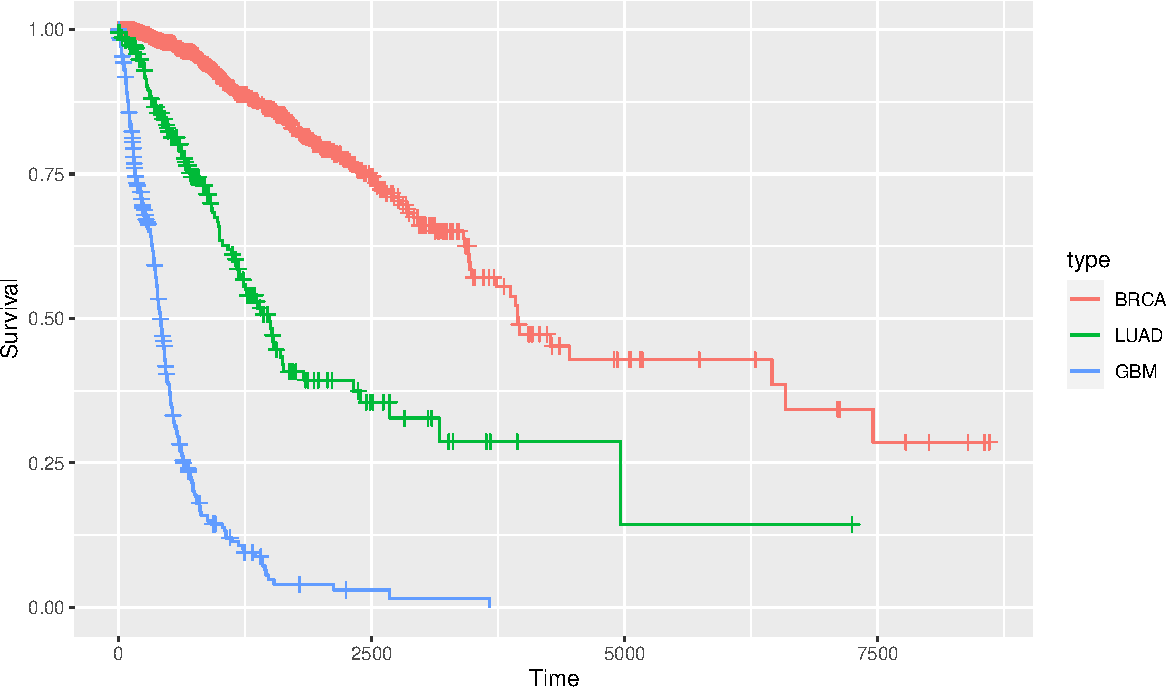
\includegraphics[width=0.8\linewidth,]{bioccb_files/figure-latex/dothesurv-1} \caption{Survival profile extraction from three MultiAssayExperiments produced with curatedTCGAData calls.}\label{fig:dothesurv}
\end{figure}

At this point, survival times within tumor type can be stratified by any
features of the mutation profiles of individual samples.
The ``RaggedExperiment'' class is employed to test each BRCA sample for
presence of any mutation in the gene TTN. See Figure \ref{fig:strat}.

\begin{verbatim}
bprim = TCGAprimaryTumors(brmut)
## harmonizing input:
##
removing 5 sampleMap rows with 'colname' not in colnames of experiments
mutsyms = assay(experiments(bprim)[[1]], "Hugo_Symbol")
cn = rownames(colData(bprim)) # short
cna = colnames(mutsyms) # long
cnas = substr(cna, 1, 12)
hasTTNmut = apply(assay(experiments(TCGAprimaryTumors(brmut))[[1]], "Hugo_Symbol"),
2, function(x) length(which(x=="TTN"))>0)
## harmonizing input:
##
removing 5 sampleMap rows with 'colname' not in colnames of experiments
names(hasTTNmut) = cnas
bsurv = getSurv(TCGAprimaryTumors(brmut))
## harmonizing input:
##
removing 5 sampleMap rows with 'colname' not in colnames of experiments
hasTTNmut = hasTTNmut[cn] # match mutation records to surv times
ggsurv(survfit(bsurv~hasTTNmut))
\end{verbatim}


\begin{figure}
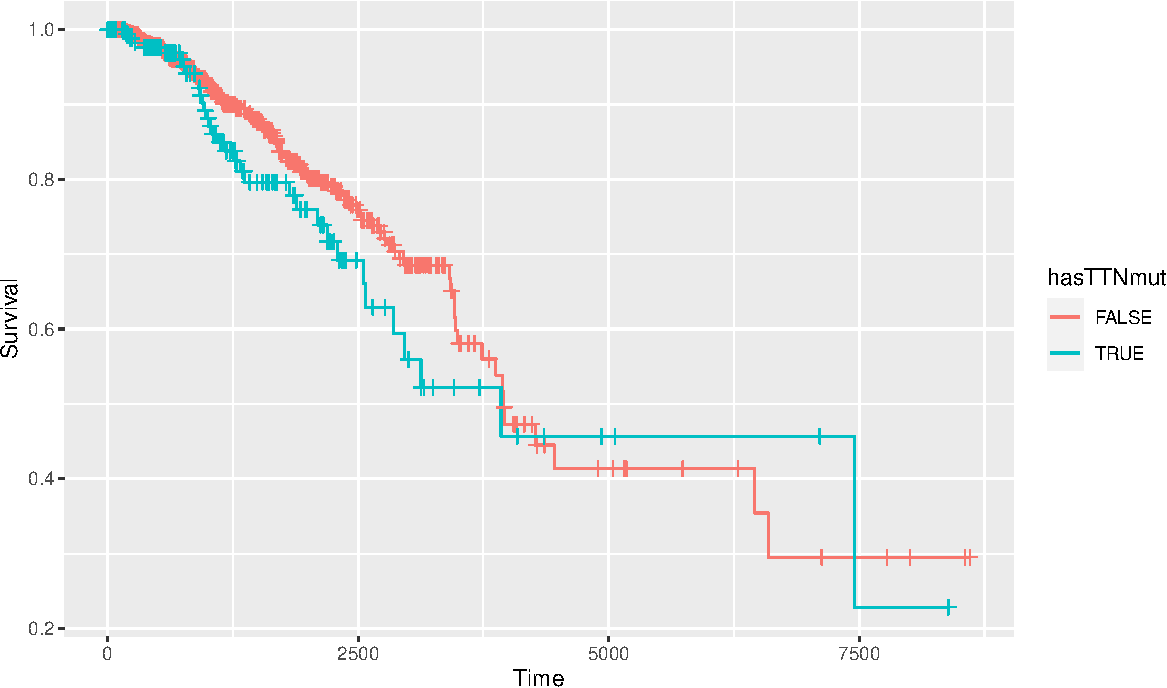
\includegraphics[width=1\linewidth,]{bioccb_files/figure-latex/strat-1} \caption{Survival distributions for donors of breast tumors in TCGA, stratified by presence or absence of mutation in gene TTN.}\label{fig:strat}
\end{figure}

Similar manipulations permit exploration of relationships between
any molecular assay outcomes and any clinical data collected in TCGA.


\subsection{cBioPortal}\label{cbioportal}}

The \href{https://www.cbioportal.org/}{cBioPortal} user guide
defines the goal of the portal to be reducing ``the barriers between complex
genomic data and cancer researchers by providing rapid, intuitive, and high-quality
access to molecular profiles and clinical attributes from large-scale cancer genomics projects, and
therefore to empower researchers to translate these rich data sets into biologic insights and clinical applications.''

Bioconductor's cBioPortalData package simplifies access to over 300 genomic studies of
diverse cancers in cBioPortal. The main unit of data access is the publication. The
\texttt{cBioPortal} function mediates a connection between an R session and the
cBioPortal API. \texttt{getStudies} returns a tibble with metadata on
all studies.

\begin{Shaded}
\begin{verbatim}
library(cBioPortalData)
cbio = cBioPortal()
allst = getStudies(cbio)
dim(allst)
## [1] 397
13
\end{verbatim}
\end{Shaded}

A pruned selection of records from the cBioPortal
studies table is given in Table \ref{tab:tab-cball}.

\begin{longtable}[t]{>{\raggedright\arraybackslash}p{12em}>{\raggedright\arraybackslash}p{15em}l}
\caption{\label{tab:tab-cball}Excerpts from four fields on selected records in the cBioPortal getStudies output.}\\
\toprule
name & description & studyId\\
\midrule
Adenoid Cystic Carcinoma of the Breast & Whole exome sequencing of 12 breast AdCCs. & acbc\_mskcc\_2015\\
Adenoid Cystic Carcinoma & Whole-exome or whole-genome sequencing analysis of 60 ACC tumor/normal pairs & acyc\_mskcc\_2013\\
Adenoid Cystic Carcinoma & Targeted Sequencing of 28 metastatic Adenoid Cystic Carcinoma samples. & acyc\_fmi\_2014\\
Adenoid Cystic Carcinoma & Whole-genome or whole-exome sequencing of 25 adenoid cystic carcinoma tumor/normal pairs. & acyc\_jhu\_2016\\
Adenoid Cystic Carcinoma & WGS of 21 salivary ACCs and targeted molecular analyses of a validation set (81 patients). & acyc\_mda\_2015\\
\addlinespace
Adenoid Cystic Carcinoma & Whole-genome/exome sequencing of 10 ACC PDX models. & acyc\_mgh\_2016\\
Adenoid Cystic Carcinoma & Whole exome sequencing of 24 ACCs. & acyc\_sanger\_2013\\
Adenoid Cystic Carcinoma Project & Multi-Institute Cohort of 1045 Adenoid Cystic Carcinoma patients. & acc\_2019\\
Basal Cell Carcinoma & Whole-exome sequencing of 126 basal cell carcinoma tumor/normal pairs; targeted sequencing of 163 sporadic samples (40 tumor/normal pairs) and 4 Gorlin symdrome basal cell carcinomas. & bcc\_unige\_2016\\
\bottomrule
\end{longtable}

To explore copy number alteration data from a study on angiosarcoma,
we find the associated studyId field in \texttt{allst} and use the \texttt{cBioDataPack} function
to retrieve a MultiAssayExperiment:

\begin{verbatim}
ann = "angs_project_painter_2018"
ang = cBioDataPack(ann)
## Warning in .find_with_xfix(df_colnames, get(paste0(fix, 1)), get(paste0(fix, :
## Multiple prefixes found, using keyword 'region' or taking first one
## Warning in .find_with_xfix(df_colnames, get(paste0(fix, 1)), get(paste0(fix, :
## Multiple prefixes found, using keyword 'region' or taking first one
ang
## A MultiAssayExperiment object of 3 listed
##experiments with user-defined names and respective classes.
####Containing an ExperimentList class object of length 3:
[1] cna_hg19.seg: RaggedExperiment with 27835 rows and 48 columns
##[2] cna: SummarizedExperiment with 23109 rows and 48 columns
##[3] mutations: RaggedExperiment with 24058 rows and 48 columns
## Functionality:
##experiments() - obtain the ExperimentList instance
##colData() - the primary/phenotype DataFrame
##sampleMap() - the sample coordination DataFrame
##`$`, `[`, `[[` - extract colData columns, subset, or experiment
####*Format() - convert into a long or wide DataFrame
assays() - convert ExperimentList to a SimpleList of matrices
##exportClass() - save data to flat files
\end{verbatim}

The copy number alteration outcomes are in the
\texttt{assay} component of the experiment.

\begin{Shaded}
\begin{verbatim}
seg = experiments(ang)[[1]]
colnames(seg) = sapply(strsplit(colnames(seg), "-"), "[", 5)
assay(seg)[1:4,1:4]
##
##                   DAE1F DACME DADBW DAD34
## 1:12227-955755       71    NA    NA    NA
## 1:957844-1139868     62    NA    NA    NA
## 1:1140874-1471177   167    NA    NA    NA
## 1:1475170-1855370   113    NA    NA    NA
\end{verbatim}
\end{Shaded}

The rownames component of this matrix can be transformed to
a GenomicRanges instance for concise manipulation.

%\begin{Shaded}
%\begin{Highlighting}[]
%\KeywordTok{library}\NormalTok{(GenomicRanges)}
%\CommentTok{\#\# 0/0 packages newly attached/loaded, see sessionInfo() for details.}
%\KeywordTok{library}\NormalTok{(ggplot2)}
%\CommentTok{\#\# 0/0 packages newly attached/loaded, see sessionInfo() for details.}
%\NormalTok{allalt =}\StringTok{ }\KeywordTok{GRanges}\NormalTok{(}\KeywordTok{rownames}\NormalTok{(}\KeywordTok{assay}\NormalTok{(seg)))}
%\NormalTok{allalt}
%\CommentTok{\#\# GRanges object with 27835 ranges and 0 metadata columns:}
%\CommentTok{\#\#           seqnames            ranges strand}
%\CommentTok{\#\#              \textless{}Rle\textgreater{}         \textless{}IRanges\textgreater{}  \textless{}Rle\textgreater{}}
%\CommentTok{\#\#       [1]        1      12227{-}955755      *}
%\CommentTok{\#\#       [2]        1    957844{-}1139868      *}
%\CommentTok{\#\#       [3]        1   1140874{-}1471177      *}
%\CommentTok{\#\#       [4]        1   1475170{-}1855370      *}
%\CommentTok{\#\#       [5]        1  1857786{-}17257894      *}
%\CommentTok{\#\#       ...      ...               ...    ...}
%\CommentTok{\#\#   [27831]       20     68410{-}1559342      *}
%\CommentTok{\#\#   [27832]       20   1585705{-}1592359      *}
%\CommentTok{\#\#   [27833]       20  1616247{-}62904955      *}
%\CommentTok{\#\#   [27834]       21  9907492{-}48084286      *}
%\CommentTok{\#\#   [27835]       22 16157938{-}51237572      *}
%\CommentTok{\#\#   {-}{-}{-}{-}{-}{-}{-}}
%\CommentTok{\#\#   seqinfo: 22 sequences from an unspecified genome; no seqlengths}
%\end{Highlighting}
%\end{Shaded}

We'll focus on chromosome 17, where TP53 is found. Regions
of genomic alteration are summarized to their midpoints.

%\begin{Shaded}
%\begin{Highlighting}[]
%\NormalTok{g17 =}\StringTok{ }\NormalTok{allalt[}\KeywordTok{seqnames}\NormalTok{(allalt)}\OperatorTok{==}\StringTok{"17"}\NormalTok{]}
%\NormalTok{df17 =}\StringTok{ }\KeywordTok{as}\NormalTok{(g17, }\StringTok{"data.frame"}\NormalTok{)        }\CommentTok{\# for ggplot2}
%\NormalTok{df17}\OperatorTok{$}\NormalTok{mid =}\StringTok{ }\FloatTok{.5}\OperatorTok{*}\NormalTok{(df17}\OperatorTok{$}\NormalTok{start}\OperatorTok{+}\NormalTok{df17}\OperatorTok{$}\NormalTok{end) }\CommentTok{\# midpoint only}
%\KeywordTok{ggplot}\NormalTok{(df17, }\KeywordTok{aes}\NormalTok{(}\DataTypeTok{x=}\NormalTok{mid)) }\OperatorTok{+}\StringTok{ }\KeywordTok{geom\_density}\NormalTok{(}\DataTypeTok{bw=}\NormalTok{.}\DecValTok{2}\NormalTok{) }\OperatorTok{+}\StringTok{ }\KeywordTok{xlab}\NormalTok{(}\StringTok{"chr 17 bp"}\NormalTok{)}
%\end{Highlighting}
%\end{Shaded}

\begin{figure}
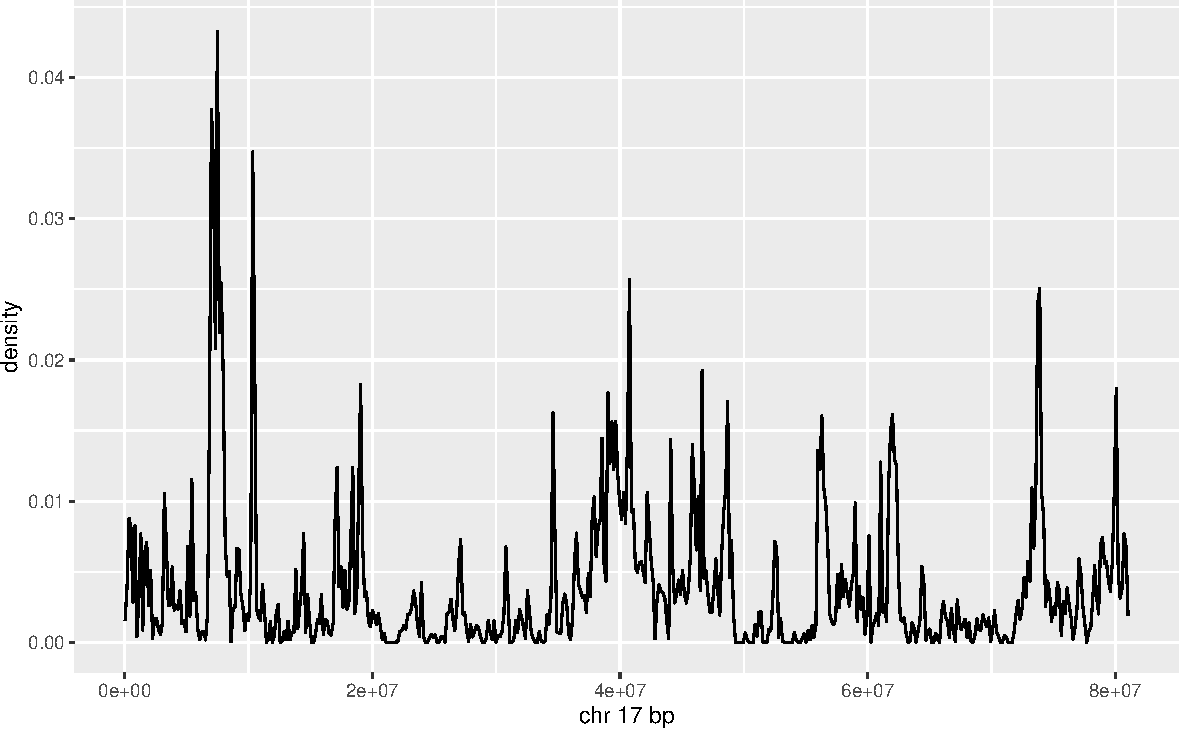
\includegraphics[width=1\linewidth,]{bioccb_files/figure-latex/mkden-1} \caption{Density of recurrent genomic alterations on chromosome 17 for 48 angiosarcoma patients.}\label{fig:mkden}
\end{figure}

This display shows a strong peak in the vicinity of 7.5 Mb on chromosome 17, near TP53.

